\chapter{Evaluation}

As of writing, \lcs is running with features developed throughout this thesis actively in use. It is deployed on an \fnoteurl{AWS}{https://aws.amazon.com/de/}{Amazon Web Service} instance and reachable via \url{https://www.scionlab.org} and \url{https://coord.scionproto.net}. Several beta testers successfully used \lcs to register, download and install their own SCION AS; not least enabled by functionality introduced as part of this thesis. These enhancements contribute to the goal of \lcs being a key component for opening up the \lee while at the same time maintaining its simplicity.


\section{Deployed Components}

The following sections evaluate the enhancements and additions described in Chapter \ref{impl} based on the effect they take on \lcs in its current state and how they are enablers for future improvements.

\subsection{Robust User Registration}
\label{eva:regi}

The process of registering an account on \lcs was greatly improved with respect to authenticity of users, by incorporating the email verification system (Section \ref{impl_email_veri}) as well as the reCAPTCHA (Section \ref{impl_capt}). This leads to better control over resources made available to users. Figure \ref{capt:veri_process} shows the new registration form with the integrated reCAPTCHA widget and the process of validating it. If a user is not exhibiting behaviour suspicious to the reCAPTCHA algorithms, no challenge is required to be solved. Therefore, this protection mechanism does not interfere with the registration process the user goes through.

\begin{figure}%captcha process
	\centering
	\subfloat[reCAPTCHA not solved]{{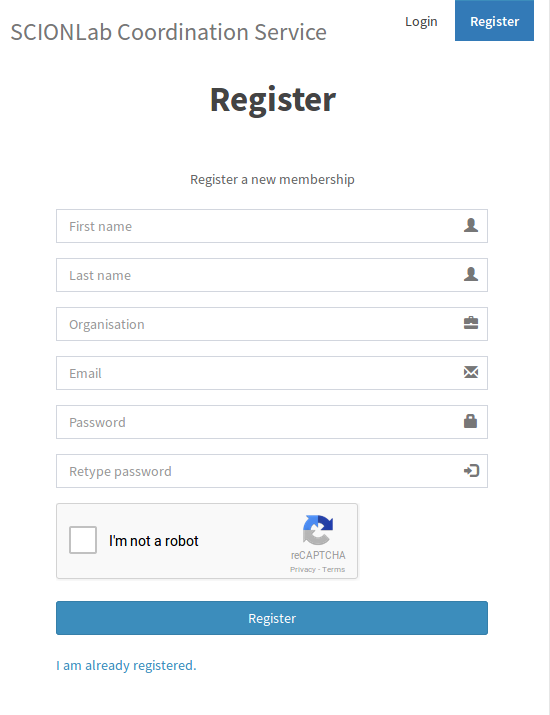
\includegraphics[width=0.33\linewidth]{captcha/captcha_empty.png} }}%
	%\qquad
	\subfloat[reCAPTCHA challenge]{{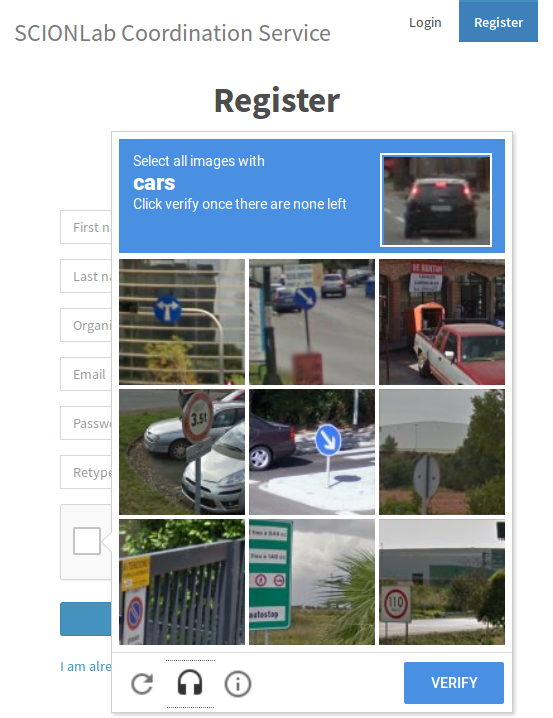
\includegraphics[width=0.33\linewidth]{captcha/captcha_challenge.png} }}%
	%\qquad
	\subfloat[reCAPTCHA solved]{{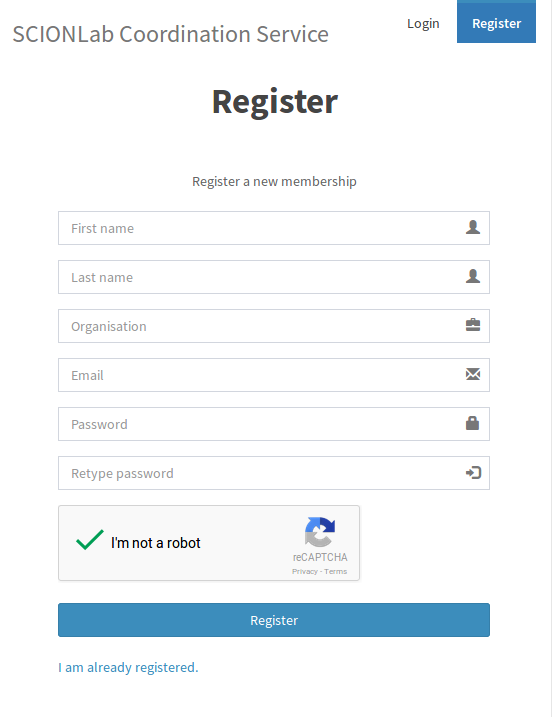
\includegraphics[width=0.33\linewidth]{captcha/captcha_verified.png} }}%
	\caption{reCAPTCHA verification process; challenge (b) is not necessary if the user behaves humanly}%
	\label{capt:veri_process}%
\end{figure}

 For users who have not been invited to use SCIONLab, a registration without solving the reCAPTCHA is not possible; neither via web interface nor by exploiting the relevant API directly. Figure \ref{veri:capt_not_solved} shows the error message presented when a user does not solve the reCAPTCHA in the registration form. Figure \ref{capt:invalid_key} shows the HTTP responses received when addressing the registration API directly; once with an invalid key and once by performing a replay attack.

\begin{figure}[h] %captcha not solved [leave away]
	\centering
	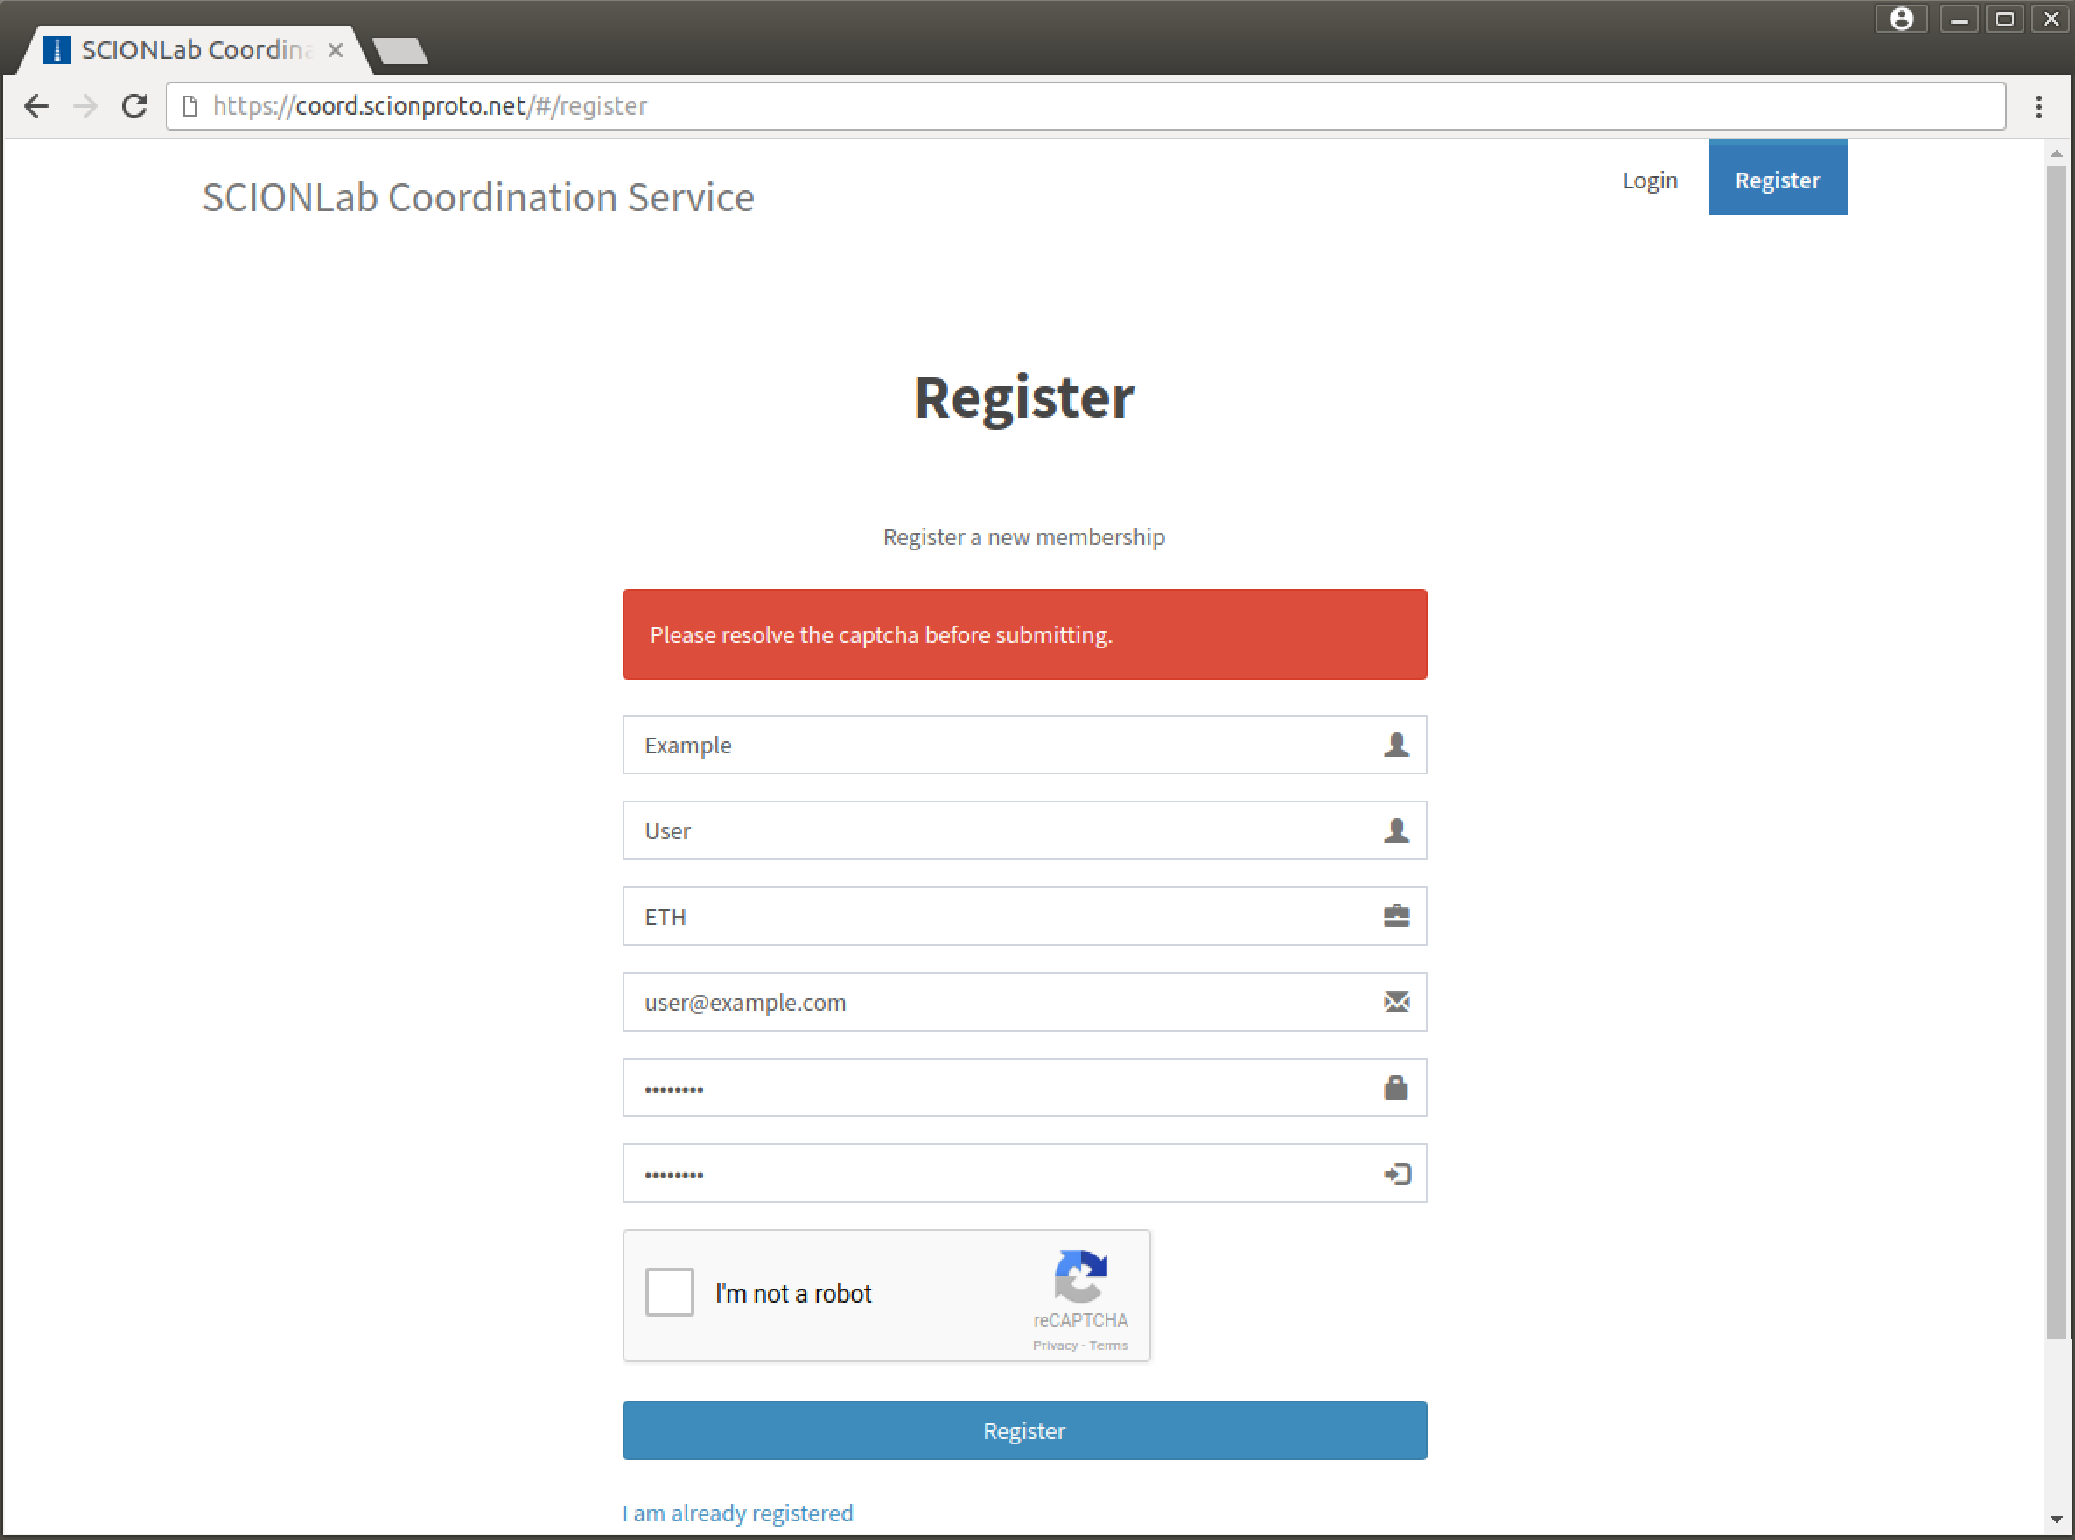
\includegraphics[width=.75\linewidth]{captcha/captcha_over_form_not_solved.png}
	\captionof{figure}{User with unsolved reCAPTCHA prevented from registering}
	\label{veri:capt_not_solved}
\end{figure}

\begin{figure}%api called directly
	\centering
	\subfloat[Invalid reCAPTCHA response key]{{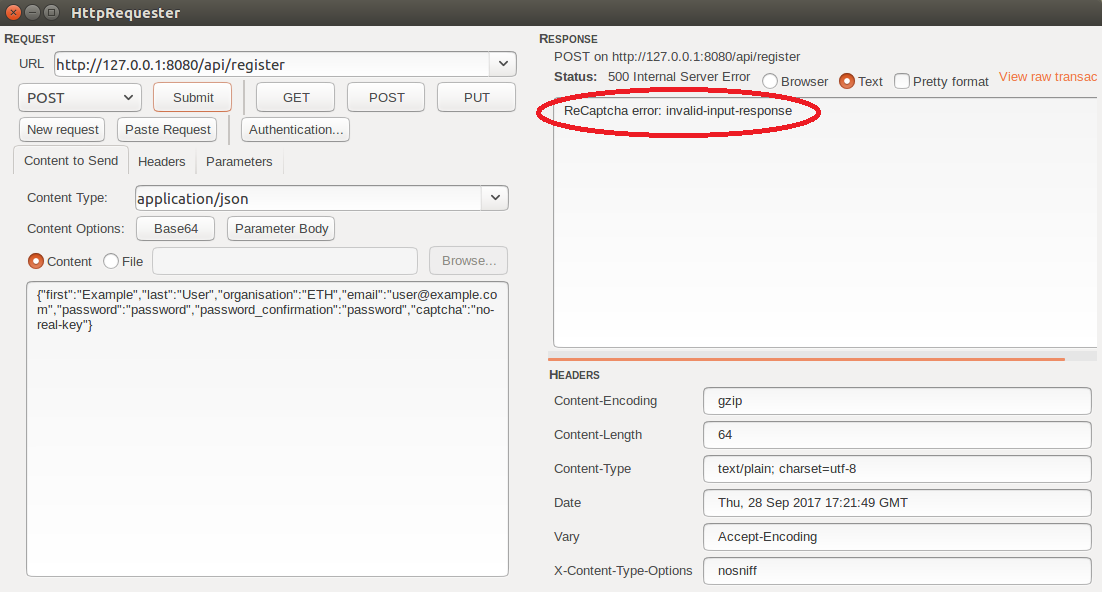
\includegraphics[width=.5\linewidth]{captcha/captcha_invalid_key.png} }}%
	%\par
	\subfloat[Duplicate reCAPTCHA response key]{{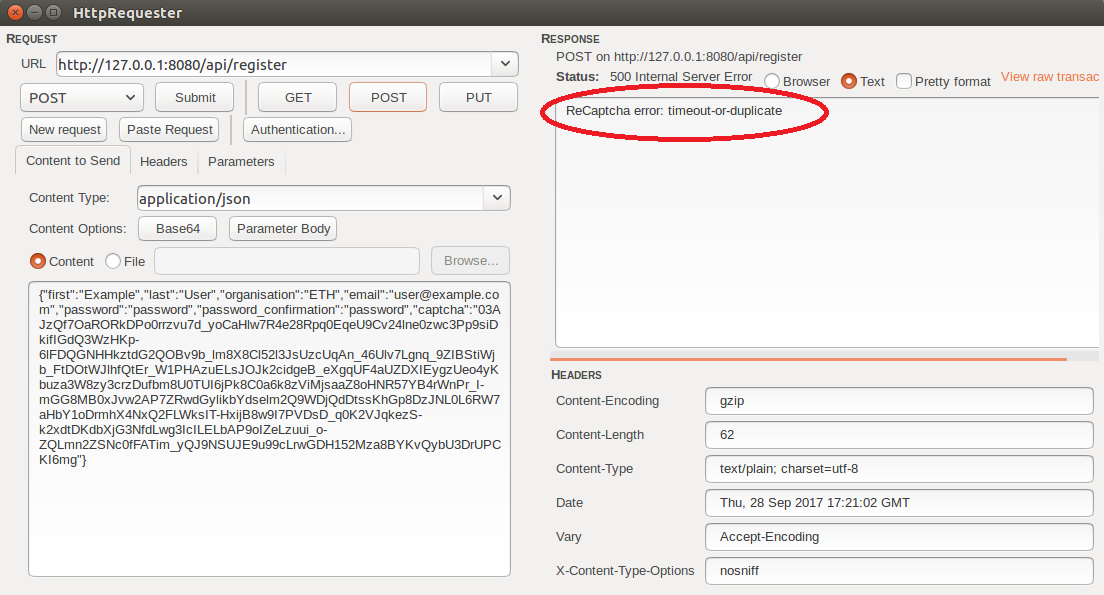
\includegraphics[width=.5\linewidth]{captcha/captcha_duplicate_key.png} }}%
	\caption{Error messages returned when trying to circumvent the reCAPTCHA with invalid or duplicate keys. The generated POST requests mimic the behaviour of a bot trying to register an account. (requests issued using \href{https://addons.mozilla.org/de/firefox/addon/httprequester/}{HttpRequester})}%
	\label{capt:invalid_key}%
\end{figure}

When a user does sign up successfully a prompt with further instructions is shown. (see Figure \ref{veri:registration_success}). Figure \ref{veri:success_and_email} shows the email containing the verification link sent to the user and the confirmation page loaded upon following the link.

\begin{figure}[h] %registration success  [leave away]
	\centering
	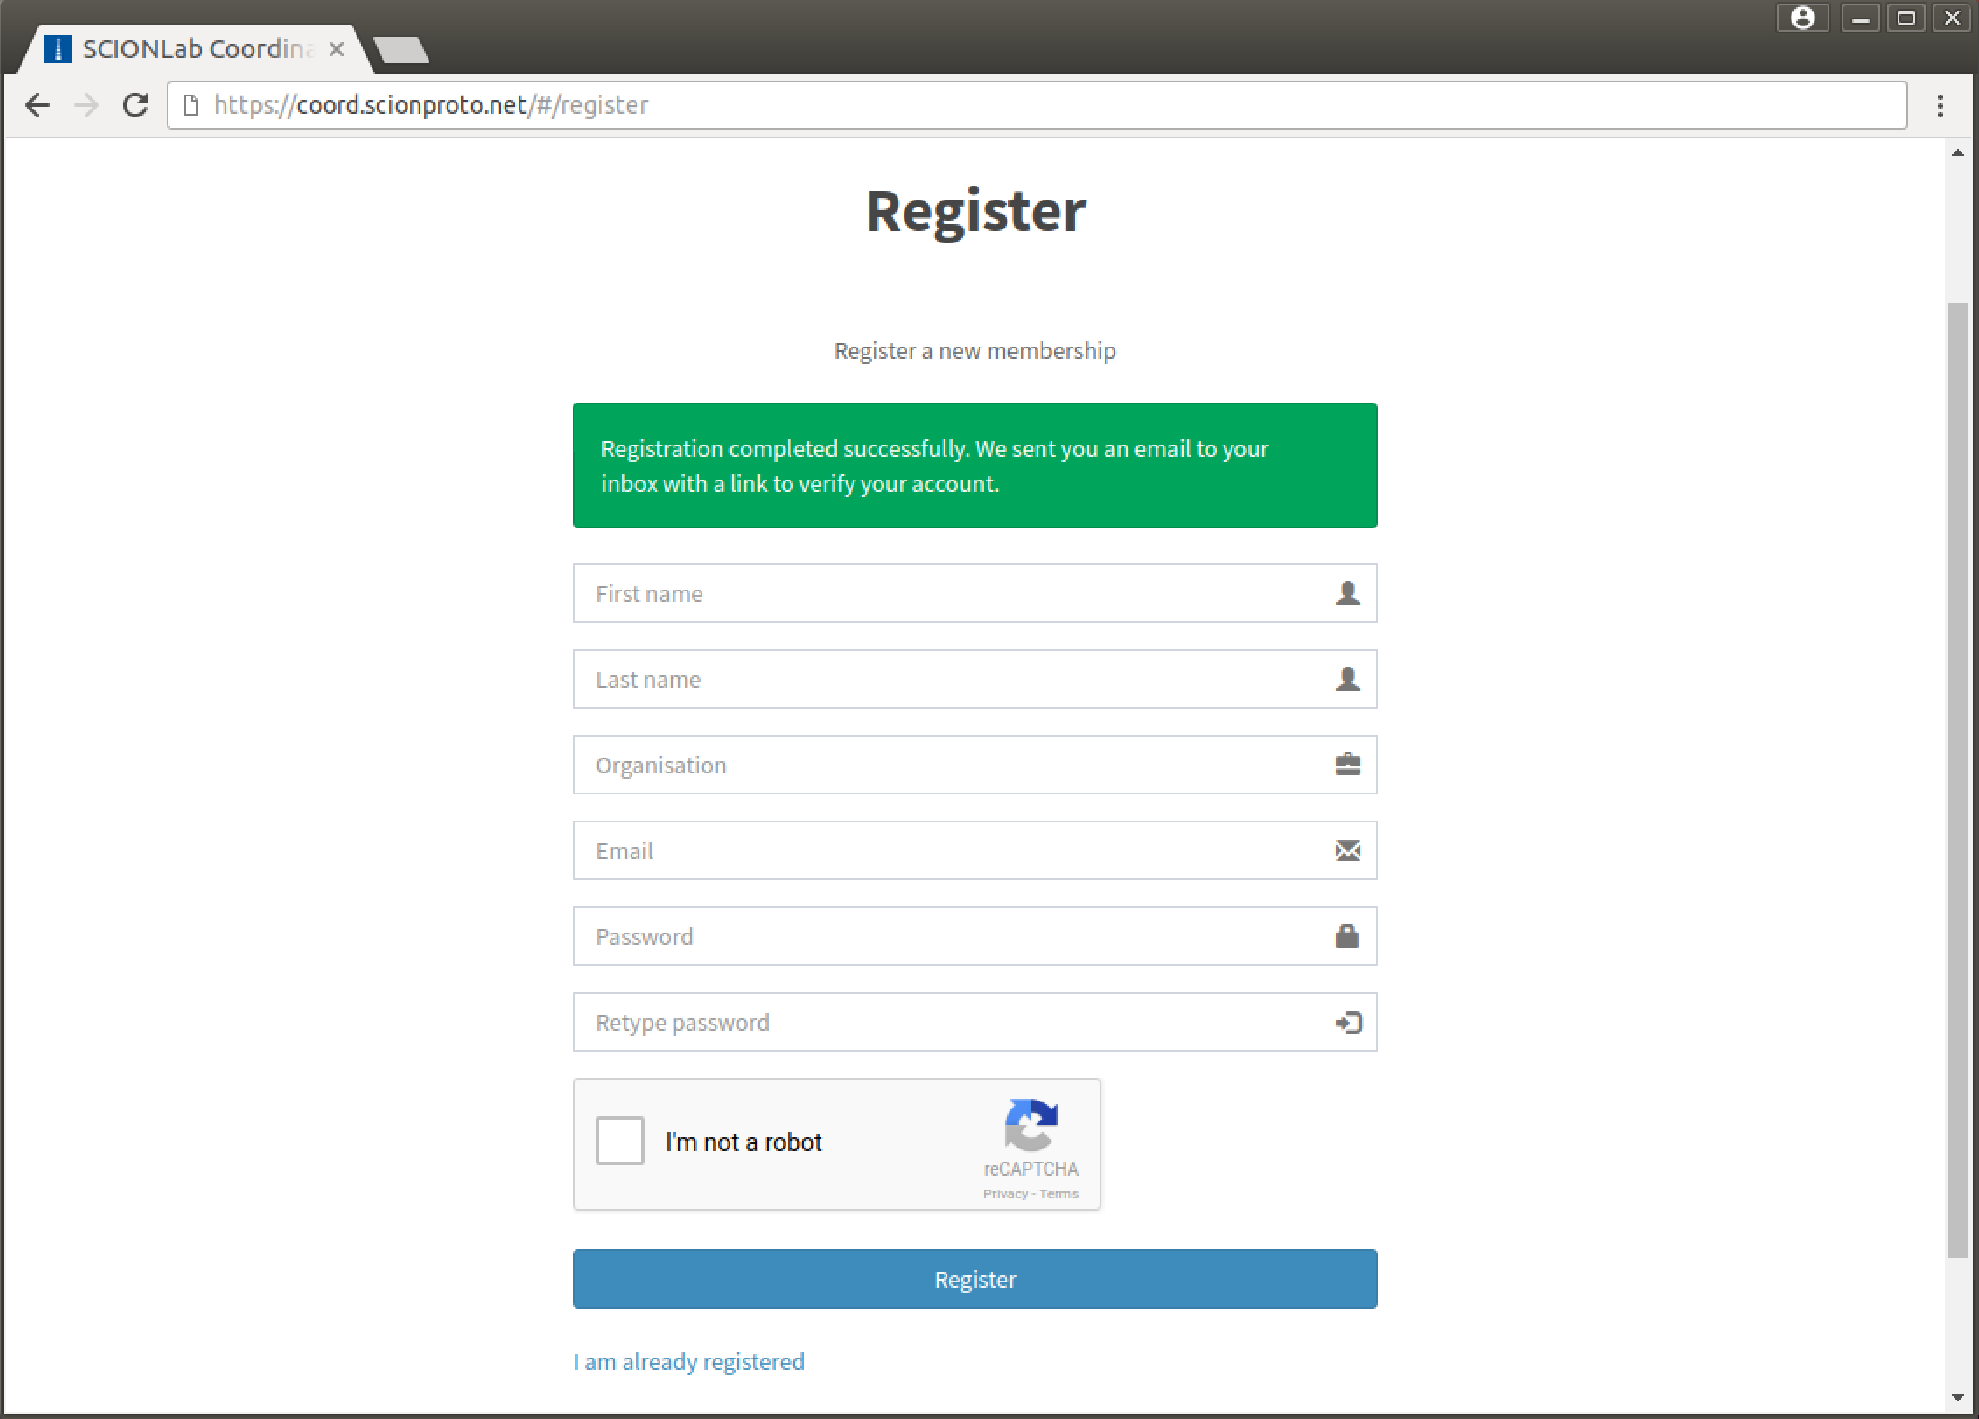
\includegraphics[width=.7\linewidth]{email_verification/email_veri_signup.png}
	\captionof{figure}{Instructions presented to users upon successful registration}
	\label{veri:registration_success}
\end{figure}

\begin{figure}[h]%verifictation email & landing page
	\centering
	\subfloat[Verification email sent to user (underlined in red the personalized identifier)]{{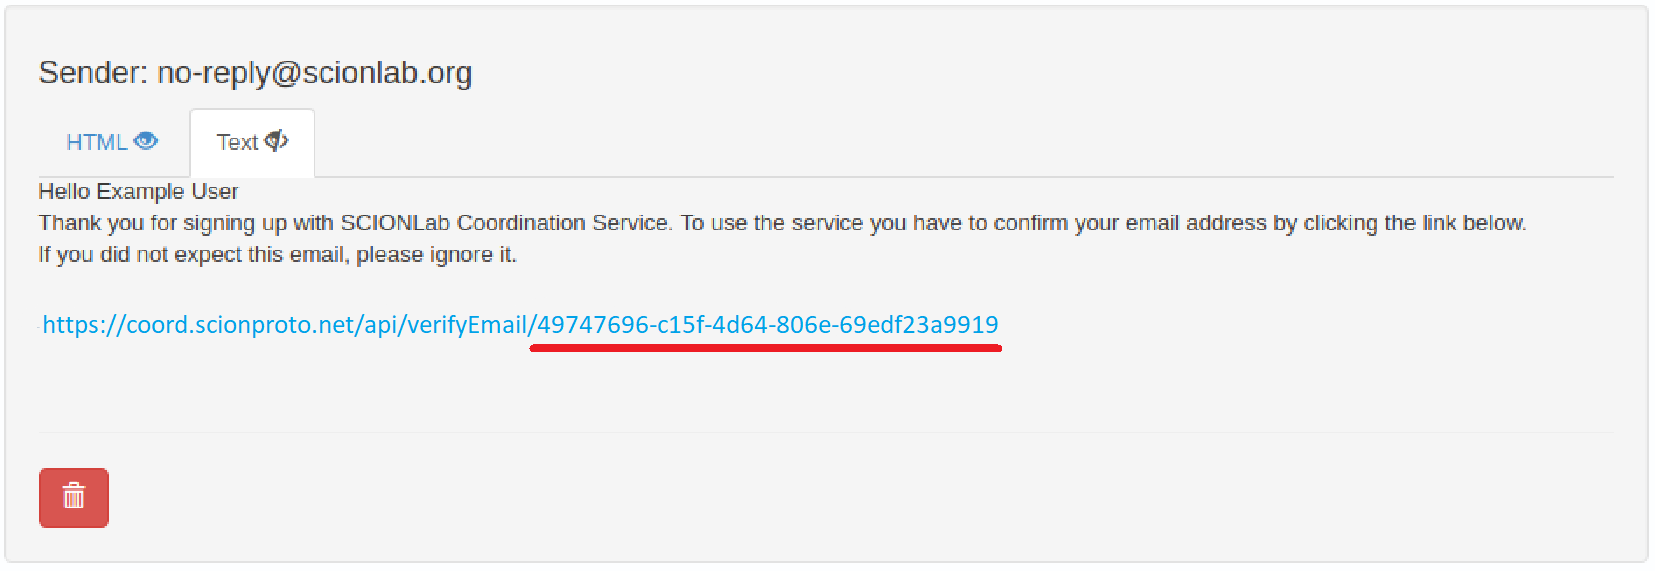
\includegraphics[width=.7\linewidth]{email_verification/email_veri_email.png} }}%
	\par
	\subfloat[Confirmation page when following personalized link]{{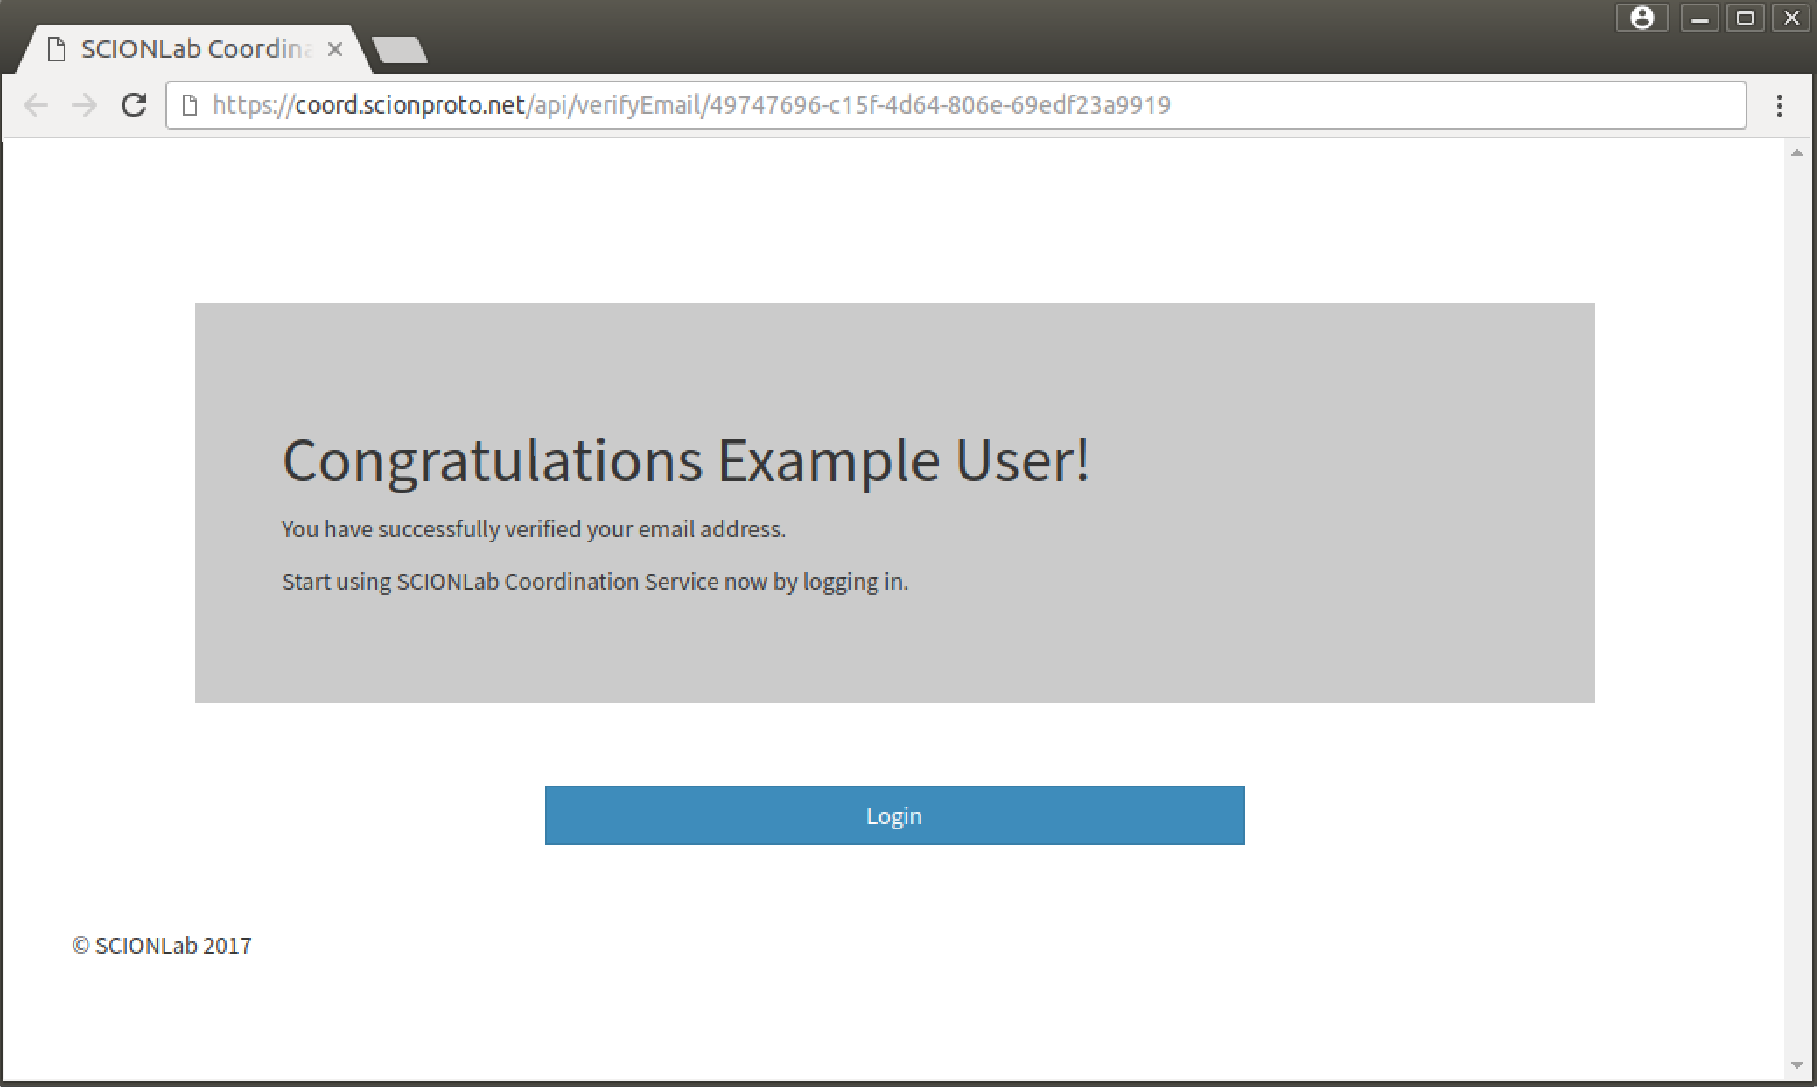
\includegraphics[width=.7\linewidth]{email_verification/email_veri_landing.png} }}%
	\caption{Email verification process with (a) email sent to user and (b) confirmation page}%
	\label{veri:success_and_email}%
\end{figure}

Users who registered with an email address that can not be verified are not granted access to \lcs. (see Figure \ref{veri:not_verified})

\begin{figure}[h]%login prevented  [leave away maybe]
	\centering
	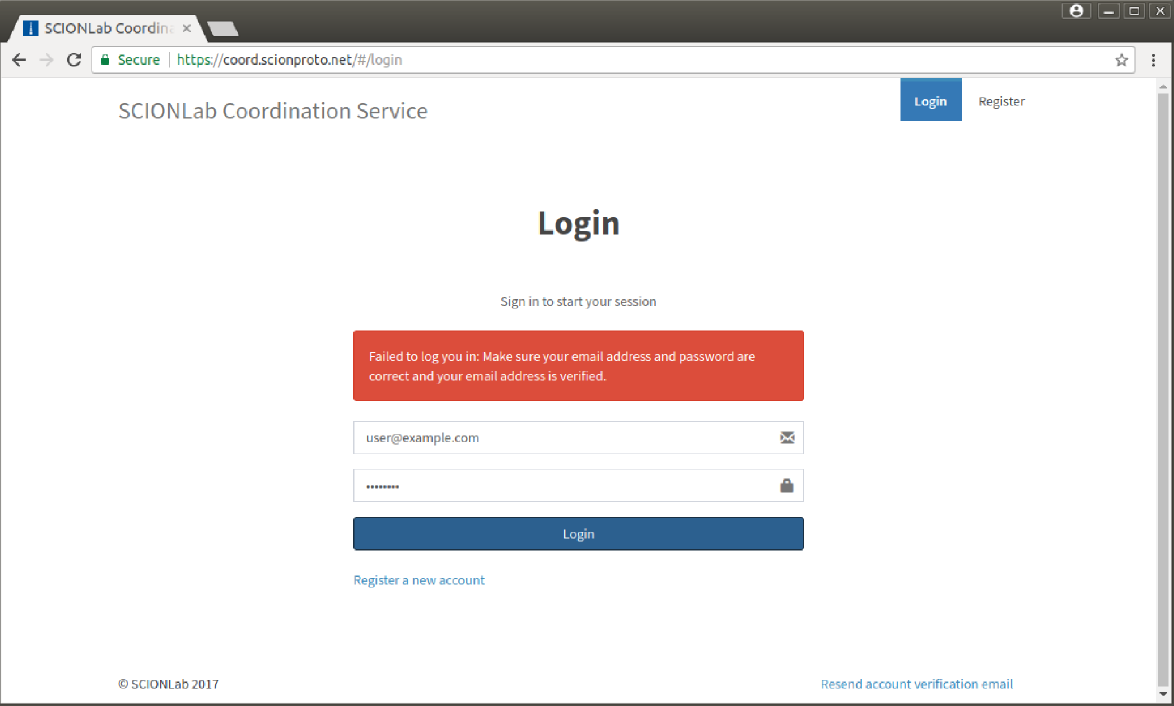
\includegraphics[width=.7\linewidth]{email_verification/email_veri_not_verfied_login.png}
	\captionof{figure}{User without verified email address prevented from logging in}
	\label{veri:not_verified}
\end{figure}

This renovated process stands in contrast to the initial basic implementation that allowed users to register with an email address they do not own or which does not exist at all. Also, by exploiting the exposed API endpoint, it was easily possible to automate the registration process in order to spam the system. Combined, the email verification system and the reCAPTCHA implementation actively prohibit system abuse.

\subsection{Invitation Based Registration}
\label{eva:invi}

The manual user activation feature outlined in Section \ref{impl_user_activation} is not being used in \lcs as of writing. The process requires new users to go through yet another round of verification. While originally intended, this proves to be cumbersome both for users as well as system administrators. Since every account has to be activated manually an administrator must log in to the administrator panel frequently in order to not cause delays. This interferes with the requirement of \lcs being a low overhead and responsive management tool. Instead, a more automated process is envisioned. Figure \ref{veri:admin_panel} shows the administrator panel for the web interface as developed for the manual user activation feature.

\begin{figure}[h] %admin panel
	\centering
	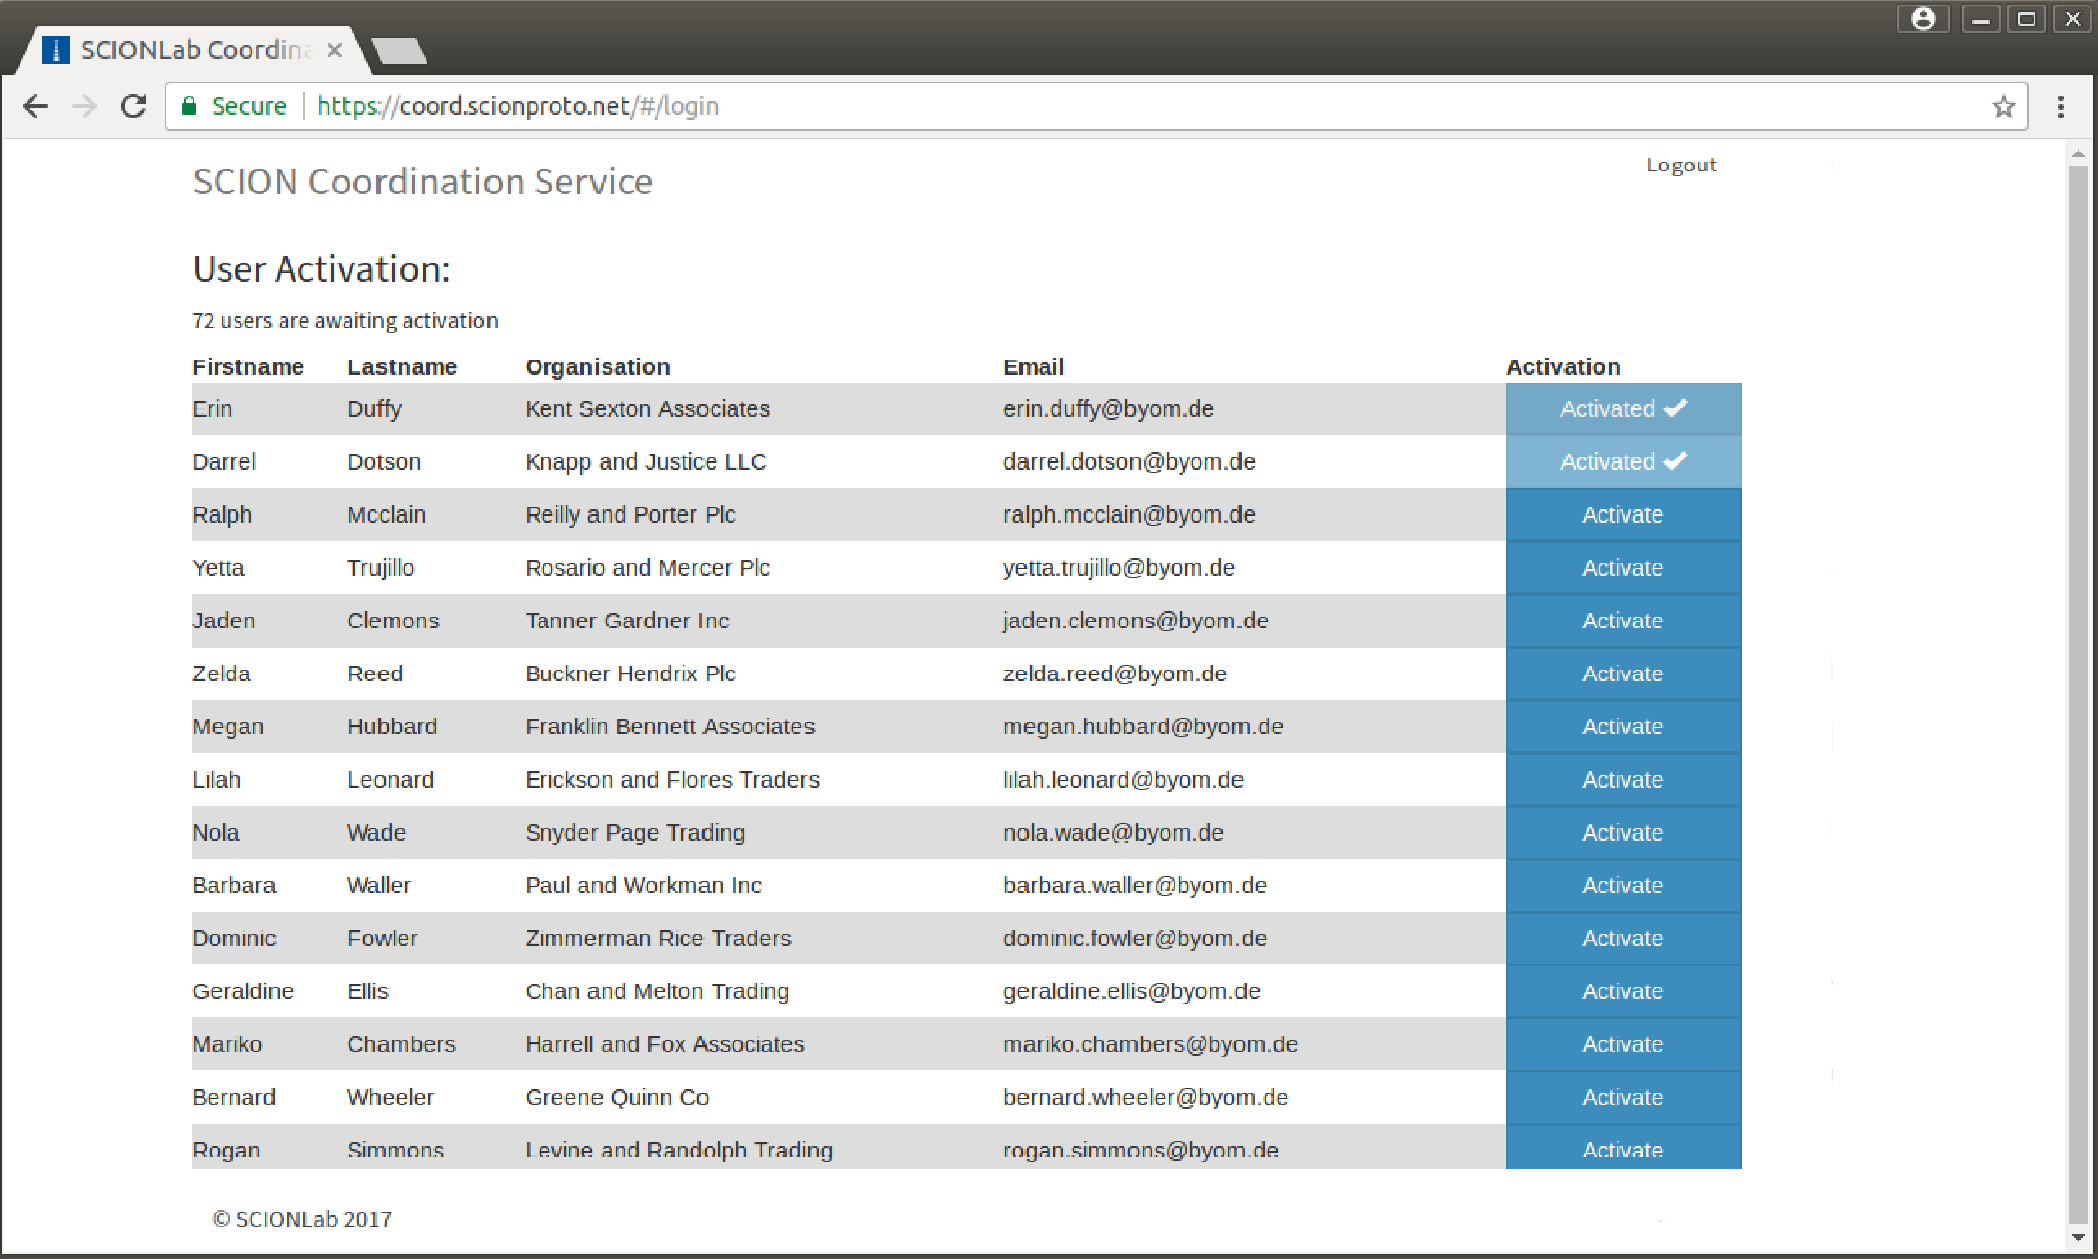
\includegraphics[width=.7\linewidth]{manual_verification/manual_veri_admin_panel.png}
	\captionof{figure}{Administrator panel on web interface used to manually activate users}
	\label{veri:admin_panel}
\end{figure}

For above reasons, core components such as the role based access control model and the administrator web panel were leveraged by the development team to build a new, invitation based registration model. Via the web panel, administrators can send out invitation emails to specific users. These users are pre-approved and do not go through a verification process.

The components developed for manual user activation  (Section \ref{impl_user_activation}) are extensible. The role based access control model provides a framework for adding additional roles with different sets of permissions to \lcs as needed. Also, the administrator panel can be extended to handle other administration related tasks. 

\subsection{Email Functionality}
\label{eva:email}

Apart from the email verification process multiple new improvements made to \lcs rely on the email package introduced in Section \ref{impl_email_package}. For one, other developers were able to implement a notification system, informing users about status changes of their running ASes. Additionally, the aforementioned invitation based registration system makes use of the email package for sending invitations to recipients.

Email sending in \lcs is easily extensible with new email templates for use in future enhancements.
The email package provides high reliability for sending transactional emails as already discussed in Section \ref{impl_email_package}. (see Figures \ref{postmark_spam} and \ref{postmark_auth})

\subsection{Integrated Testing}
\label{eva:test}

CircleCI integration (Section \ref{impl_ci}) has been set up for \lcs and used by the development team to validate code contributions. Currently, the test suite of \lcs consists of 3 unit tests with a total of 15 test cases. CircleCI takes 45-70 seconds to process these tests. This includes building the environment, downloading source code and dependencies and then running the tests. Figure \ref{ci:failed} shows the output generated for a failed test on CircleCI.

This integration does not require any work for adding additional tests, apart from writing the tests themselves, as they will be picked up and run by CircleCI automatically.

\begin{figure}[h] %admin panel
	\centering
	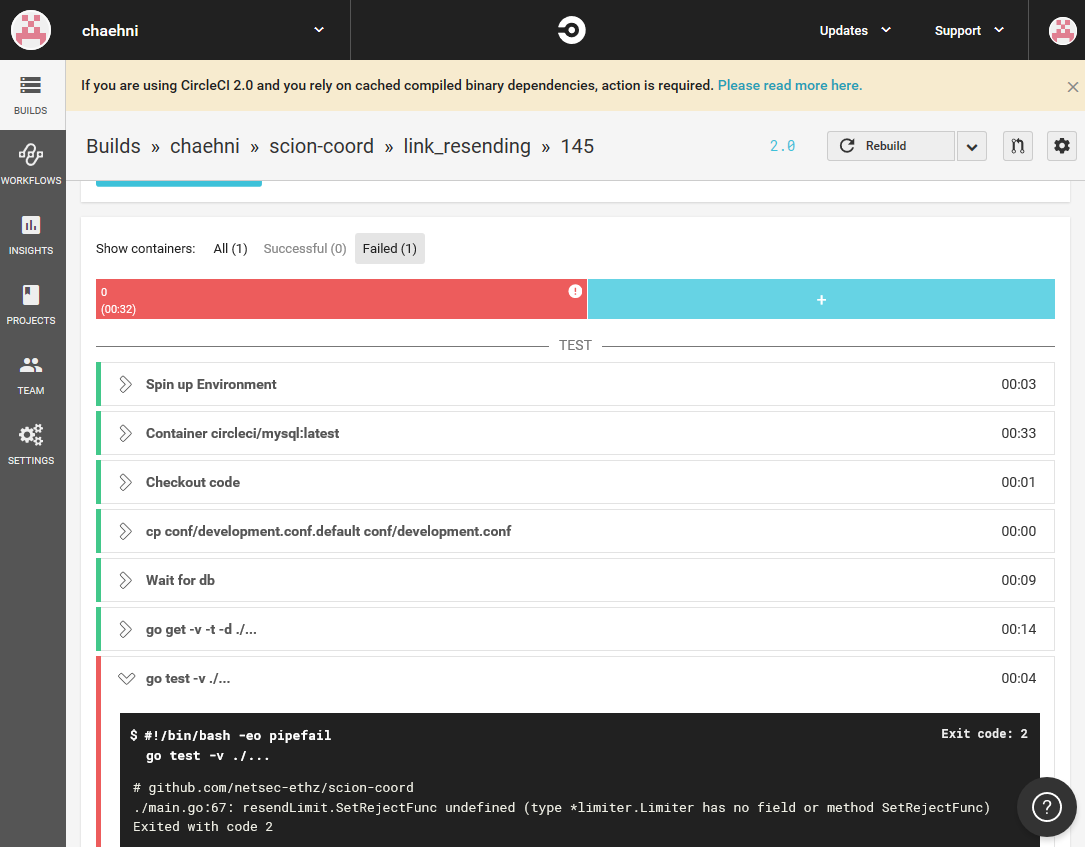
\includegraphics[width=.7\linewidth]{circleci/ci_failed.png}
	\captionof{figure}{Failed test on CircleCI}
	\label{ci:failed}
\end{figure}

%\begin{figure} %admin panel
%	\centering
%	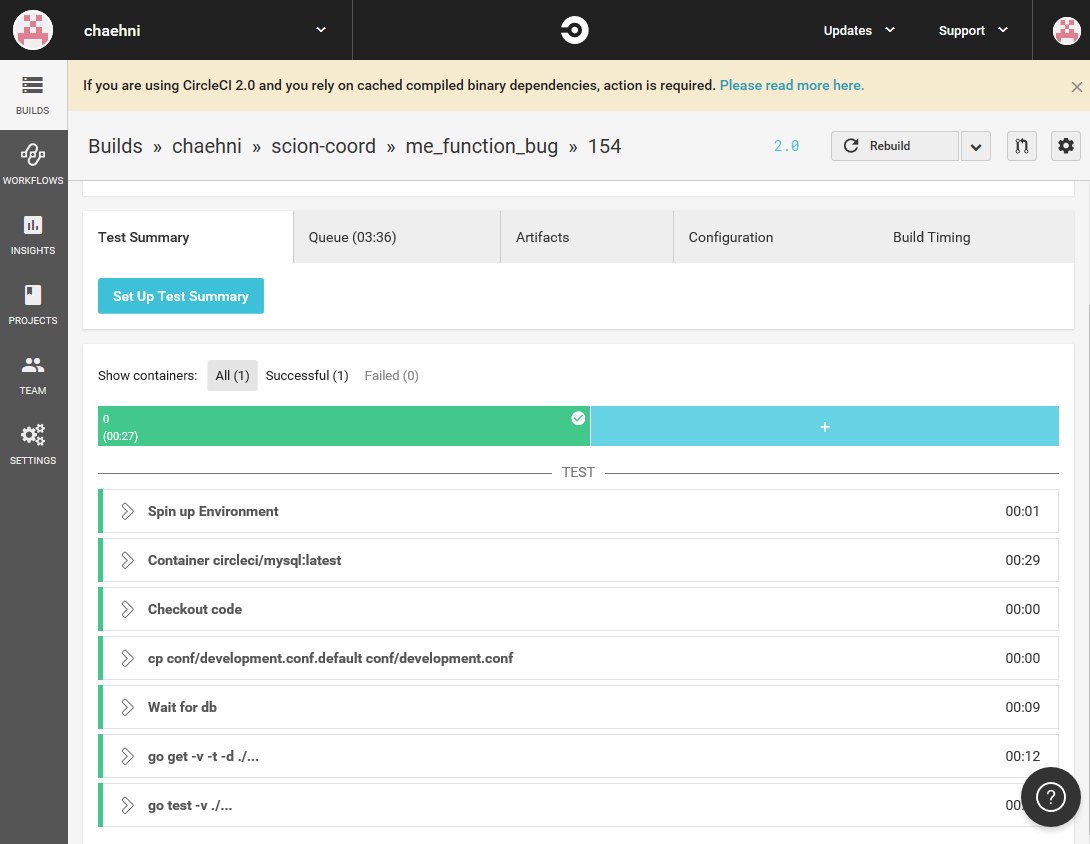
\includegraphics[width=\linewidth]{circleci/ci_success.png}
%	\captionof{figure}{Successful test on CircleCI}
%	\label{ci:success}
%\end{figure}

\subsection{Effortless Deployment}
\label{eva:deploy}

The Ansible playbook for smooth deployment of \lcs onto remote machines was successfully used throughout this thesis to deploy newly developed code onto an AWS instance set up for testing purposes. However, the playbook has not been used in production. In the meantime adjustments are necessary to adapt the playbook to the fast evolving \lcs code base. The reason these adjustments are necessary is that changes made to the service have not been reflected in the Ansible playbook. Most notably, Ansible must be advised to install additional files, such as encryption keys for VPN based connections, to produce the required environment for the service to function correctly with newly introduced VPN connections. 

Nonetheless, if maintained, the framework provided could prove useful for future deployments, especially when moving towards a replicated set up of \lcs where, manual deployment becomes too time consuming.

\section{Requirements Evaluation}

This section summarizes to what extent the requirements gathered in Chapter \ref{req} have been satisfied by the work done in this thesis.

\subsubsection{Functional Requirements}

\begin{enumerate}  
	\item\textit{A mechanism to verify users' email addresses:}\\	
		This requirement is considered achieved by implementation of the email address verification system. (Section \ref{impl_email_veri}). The evaluation of this system has been discussed as part of Section \ref{eva:regi}
	\item\textit{A mechanism to manually activate users who signed up successfully:}\\
		A mechanism satisfying this requirement has been implemented (Section \ref{impl_user_activation}). Even tough the feature has not been deployed, for reasons depicted in Section \ref{eva:invi}, it nonetheless had been functional and, more importantly, provided components to be reused for the invitation based registration process. Therefore, this requirement has been achieved.
	\item\textit{A mechanism to protect the service against automated account creation:}\\
		This feature has been implemented as presented in Section \ref{impl_capt} and its functional evaluation has been shown in Section \ref{eva:regi}. This requirement is thereby fully achieved.
	\item\textit{New functionality is validated using CircleCI's testing environment:}\\
		Implemented (Section \ref{impl_ci}) and deployed, this functionality has been proven to work as described in Section \ref{eva:test}. By these means, the requirement is regarded as fulfilled.
	\item\textit{A fast and easy way to deploy the service onto multiple machines:}\\
		An Ansible playbook had been designed (Section \ref{impl:ansi}) and successfully used to deploy \lcs onto remote machines (Section \ref{eva:deploy}). Newer changes introduced to \lcs, however, have not considered adapting the playbook accordingly. This has left it in a state where it needs adjustments to be fully functional again. 
	\item\textit{A system for sending notifications to users:}\\
		By implementing the package for sending emails (Section \ref{impl_email_package}) the foundation for this requirement had been laid. However, as mentioned in Section \ref{eva:email}, the remaining parts have been added by other developers, not part of this thesis. While overall fulfilled, only parts of the solution have been provided by this thesis.
	\item\textit{Implementation of missing APIs between \cords and the \lmi:}\\
		No work has been done with respect to this requirement throughout this thesis. Therefore, it has not been achieved.
	\item\textit{A visualization of the SCIONLab Experimentation network accessible by users:}\\
		This requirement has not been worked on and is as a consequence not achieved by this thesis.
\end{enumerate}

\subsubsection{Non-Functional Requirements}

For the non-functional evaluation, rather than specifying whether or not requirements have been achieved, we are interested in what effect changes made to \lcs have on the given constraints.

\begin{enumerate}
	\item\textit{\lcs aims to be an easy to use tool:}\\
		The improved registration process (functional evaluation in Section \ref{eva:regi}) makes the process of registering an account slightly more involved. Apart from that, no changes have been made regarding ease of use. Overall, \lcs retains its simplicity.
				
	\item\textit{None of its functionality should require the user to invest a great amount of work:}\\
		The introduction of the email verification process (Section \ref{impl_email_veri}) increases the overhead for users by requiring them to check their email inbox. While making use of email callback verification (see Section \ref{impl_email_package}) would have led to less overhead, this solution has been deemed infeasible because of its unreliability. The approach taken is considered the right balance between simplicity and reliability of the feature.
		
		The CAPTCHA provider has been chosen with the goal of simplicity in mind. As described in Section \ref{eva:regi}, reCAPTCHA does not require users to invest a great amount of work.
	\item\textit{It is preferred to hide as much complexity as possible from users:}\\
		All implementations made have been designed to require as little user interaction as possible. As a result, the complexity of added features is mostly hidden from users. An exception is the email verification system which has been discussed above.
	\item\textit{The web interface of the service is required to be fast, clean and responsive, since 	it will be amongst the first impressions users get of SCION:}\\
		Apart from the added reCAPTCHA widget, the visual appearance of \lcs has not been altered by changes made in this thesis. It therefore remains clean and user-friendly.	
	\item\textit{The web interface needs to be visually appealing, both on desktop and mobile devices:}\\
		There have been no changes made regarding visual appearance on different screen sizes in this thesis.
	\item\textit{In terms of maintainability, \lcs aims for easy extensibility as the project evolves 	fast and new requirements need to be integrated with minimal effort:}\\
		As described in Appendix \ref{misc}, a variety of improvements have been made with respect to maintainability. Additionally, the implemented components (Chapter \ref{impl}) reduce the complexity for developing future extensions.
		
\end{enumerate}